\chapter{Cobertura de la demanda. Mercado eléctrico.}
\section{Explotación del mercado eléctrico.}
La energía eléctrica se genera en grandes concentradas de forma concentrada y posteriormente se transmite a grandes distancias donde el equilibrio se obtiene de las curvas de oferta y demanda.


Una misión importante de la red es la de ajustar la energía generada a la demandada con unos valores de tensión (Control Q-U) y frecuencia (Control P-f).
\section{Curva de demanda diaria.}
La demanda varia constantemente tanto hora a hora como diariamente. Esta demanda se refleja en las curvas de carga o demanda donde la diferencia entre ambas equivale a las pérdidas en la red ($\approx$12\%).

\begin{itemize}
	\item [-]\textbf{Energía producida:} se entiende en barras de la central, descontando el autoconsumo.
	\item [-]\textbf{Energías consumida:} se obtiene de la suma del consumo de los abonados.
\end{itemize}
\begin{figure}[H]
	\begin{minipage}{0.5\linewidth}
		\centering
		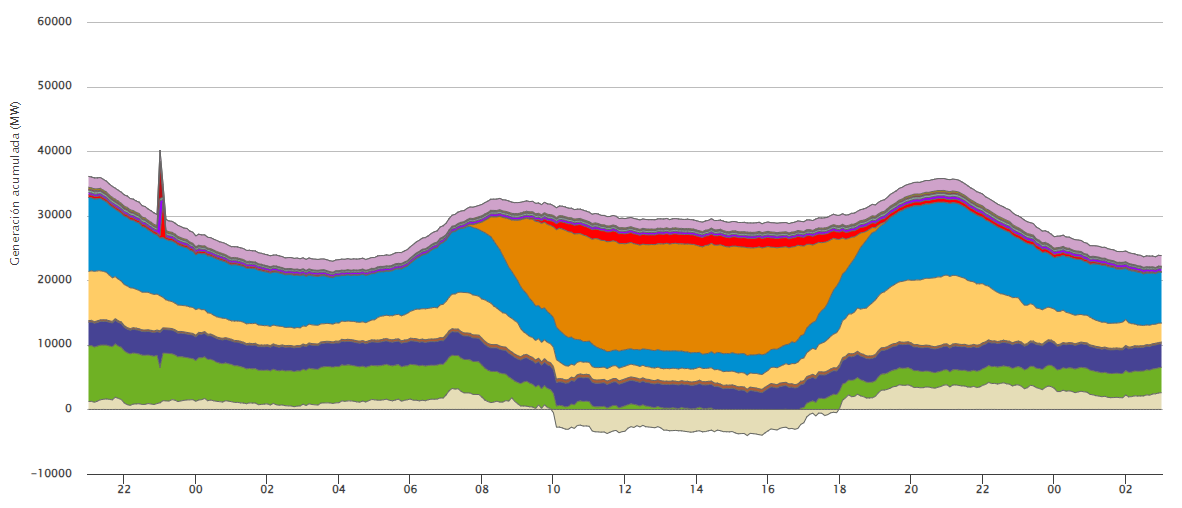
\includegraphics[width=0.7\linewidth]{res/tema4/demandaDia}
		\label{fig:demandadia}
	\end{minipage}
	\begin{minipage}{0.5\linewidth}
		\centering
		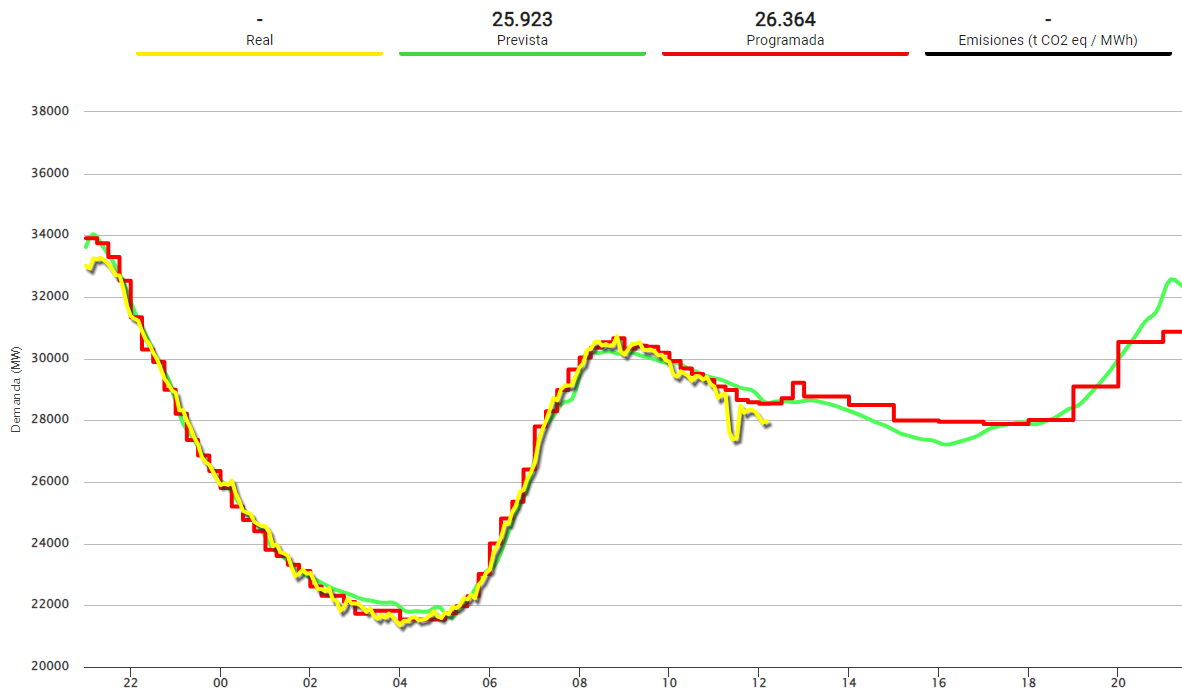
\includegraphics[width=0.7\linewidth]{res/tema4/demandaDia1}
		\label{fig:demandadia1}
	\end{minipage}
\end{figure}
La curva de carga o de demanda se predice mediante la estadística acumulada de muchos años ya que para fijar el precio es necesaria esta previsión (tiene un error asociado del 2\%). En estos datos, se pueden apreciar típicamente tres picos de consumo (12, 16 y 20 horas) que llevan a la tarifa PVPC (Precio de venta al pequeño consumidor) con discriminación horaria en horas valle, llano y punta.


Cabe destacar, como los factores locales tienen mucho peso sobre la demanda real como la temperatura, grandes eventos, ...

\section{Pérdidas en la red.}
Son un coste de operación necesario para mover la energía desde donde se produce (Galicia y Cataluña como pozos) hacia donde se consume (Madrid y Barcelona como sumideros). 
\begin{itemize}
	\item [-] Red de transporte 1-2\%
	\item [-] Red de distribución 4-6\%
	\item [-] Red baja tensión 7-10\%
\end{itemize}
\section{Gestión de la red.}
La empresa encargada de la gestión de la red es Red Eléctrica Española (REE) que recibe a través de su red de fibra óptica las potencias activa y reactiva en varios puntos de la red. La gestión se realiza desde el Centro de Control Eléctrico (CECOEL).

Para realizar esta gestión REE debe tener en cuenta muchas incertidumbres asociadas a defectos en generadores y la red lo cual provoca un sobredimensionamiento del sistema.
\subsection{Incidencias no previstas.}
Cuando ocurren incidencias graves, normalmente asociadas a una falta en la generación REE debe aplicar cortes a las industrias acogidas a contratos de interrumpibilidad.
\subsection{Configuración sistema eléctrico de potencia.}
El sistema léctrico de potencia se compone de lo siguientes elementos:
\begin{itemize}
	\item [-] \textbf{Generación:} Se genera en barras del generador de 6-30 kV a 50Hz con potencias de hasta 1500 MVA.
	\item [-] \textbf{Redes de Transporte:} Esta formada por un elevado número de nodos con topología mallada a los que se conectan los generadores y consumidores a una tensión de 220-400kV.
	\item [-] \textbf{Redes de Distribución:}  Las longitudes de estas líneas no superan los 25 km y normalmente son aéreas. En núcleos urbanos suelen ser malladas y en zona rural radiales. Se distribuye de 132-15kV.
	\item [-] \textbf{Centros de transformación:} Se reduce la tensión de media a baja tensión.
	\item [-] \textbf{Consumidores:} Red de distribución a 230/400V.
\end{itemize}
\section{Funcionamiento del mercado eléctrico.}
Desde la Ley 54/1997 se liberalizó el sector eléctrico para permitir la libre competencia con las siguientes características:
\begin{itemize}
	\item [-] Libertad de construcción de nuevas centrales de producción de electricidad.
	\item [-] Competencia entre las empresas productoras de electricidad en un mercado de ofertas.
	\item [-] Libertad progresiva de los consumidores para elegir el suministrador que deseen y acordar con
	él las condiciones y precio del kWh.
	\item [-] Libertad de comercialización de la electricidad.
	\item [-] Libertad de comprar o vender electricidad a empresas y consumidores de otros miembros de
	la UE.
	\item [-] Separación jurídica de actividades:
	\begin{itemize}
		\item \textbf{Reguladas:} transporte, distribución y gestión del sistema.
		\item \textbf{No reguladas:} generación y comercialización
	\end{itemize}
	\item [-] Sostenibilidad económica y financiera:
	\begin{itemize}
		\item Garantizar el suministro al mínimo coste.
		\item Retribución de actividades con base en criterios objetivos, transparente y homogéneos.
		\item Marco normativo que garantice la estabilidad financiera.
		\item  Actualización de los peajes de acceso a través de cargos.
	\end{itemize}
\end{itemize}
La explotación del mercado eléctrico se realiza conjuntamente entre:
\begin{itemize}
	\item 
	\item
	\item
\end{itemize}
\subsection{Actividades principales.}
g
\subsection{Reparto de la distribución de energía eléctrica.}
g
\subsection{Comercialización.}
g
\subsection{Organización.}
g
\subsection{Instituciones reguladoras.}
g
\subsection{Operador del mercado (OMIE).}
g
\subsection{Operador del sistema (REE).}
g
\section{Mercado ibérico (MIBEL).}
g
\section{Interconexiones con el extranjero.}
g
\subsection{Francia.}
g
\subsection{Portugal.}
g
\subsection{Marruecos.}
g
\subsection{Gestión de las interconexiones.}
g
\section{Mercado intradiario.}
g
\subsection{Secuencia de los procesos del mercado.}
g
\subsection{Mercados a plazo.}
g
\subsection{Mercado organizado diario (casación horaria).}
g
\subsection{Tipos de oferta de venta de energía.}
g
\subsection{Proceso de casación.}
g
\subsection{Curva de oferta de venta de energía.}
g
\subsection{Influencia fuentes renovables.}
g
\subsection{Retribuciones para amortizar costes fijos.}
g
\subsection{Curva de demanda.}
g
\section{Mercado de restricciones técnicas.}
g
\section{Mercado de servicios complementarios.}
g
\subsection{Regulación primaria.}
g
\subsection{Regulación secundaria.}
g
\subsection{Control de tensión.}
g
\subsection{Reservas de potencia.}
g
\subsection{Gestión de desvíos.}
g
\subsection{Regulación terciaria.}
g
\section{Precio medio final.}
g
\subsection{Costes recogidos en la tarifa eléctrica (PVPC).}
g
\section{Programación de la generación de electricidad.}
g
\subsection{Curva acumulada de demanda anual.}
g
\subsection{Curva de demanda anual.}
g
\subsection{Parámetros principales curva de demanda.}
g
\subsection{Curva acumulada de generación anual.}
g
\subsection{Parámetros principales curva de generación.}
g
\section{Reserva de potencia.}
g
\subsection{Características estáticas.}
g
\subsection{Características dinámicas.}
g
\subsection{Secuenciamiento óptimo de grupos.}
g
\section{Costes de generación.}
g
\subsection{Comparativa de costes.}
g
\subsection{Coste de inversión o fijo.}
g
\subsection{Costes variables.}
g
\subsection{Coste total.}
g
\section{Aspectos técnicos de la producción de energía.}
g